\documentclass[letterpaper,11pt]{article}
\usepackage{graphicx}
\usepackage{listings}
\usepackage[super]{nth}
\usepackage[hyphens]{url}
\usepackage{hyperref}
\usepackage{amsmath}
\usepackage[makeroom]{cancel}
\usepackage[table]{xcolor}
\usepackage{comment}
\usepackage[space]{grffile}
\usepackage{csvsimple}
\usepackage{longtable}


\newcommand*{\srcPath}{../src}%

\lstset{
	basicstyle=\footnotesize,
	breaklines=true,
}

\begin{document}

\begin{titlepage}

\begin{center}

\Huge{Assignment 9}

\Large{CS 532:  Introduction to Web Science}

\Large{Spring 2017}

\Large{Grant Atkins}

\Large Finished on \today

\end{center}

\end{titlepage}

\newpage


% =================================
% First question
% =================================
\section*{1}

\subsection*{Question}

\begin{verbatim}
1.  Create a blog-term matrix.  Start by grabbing 100 blogs; include:

http://f-measure.blogspot.com/
http://ws-dl.blogspot.com/

and grab 98 more as per the method shown in class.  Note that this
method randomly chooses blogs and each student will separately do
this process, so it is unlikely that these 98 blogs will be shared
among students.  In other words, no sharing of blog data.  Upload
to github your code for grabbing the blogs and provide a list of
blog URIs, both in the report and in github.

Use the blog title as the identifier for each blog (and row of the
matrix).  Use the terms from every item/title (RSS) or entry/title
(Atom) for the columns of the matrix.  The values are the frequency
of occurrence.  Essentially you are replicating the format of the
"blogdata.txt" file included with the PCI book code.  Limit the
number of terms to the most "popular" (i.e., frequent) 1000 terms,
this is *after* the criteria on p. 32 (slide 7) has been satisfied.
Remember that blogs are paginated. 
\end{verbatim}

\clearpage
\subsection*{Answer}



\begin{table}[htb]
\centering
\begin{tabular}{ | l | l | l | l |}
\hline
\textbf{Source User} & \textbf{Target User} & \textbf{Following Target} & \textbf{Followed By Target} \\
\hline
\end{tabular}
\caption{Format of friendships.csv, where Following fields are booleans}
\label{table:q1csvtable}
\end{table}



\clearpage
 \begin{figure}[h]
 \centering
 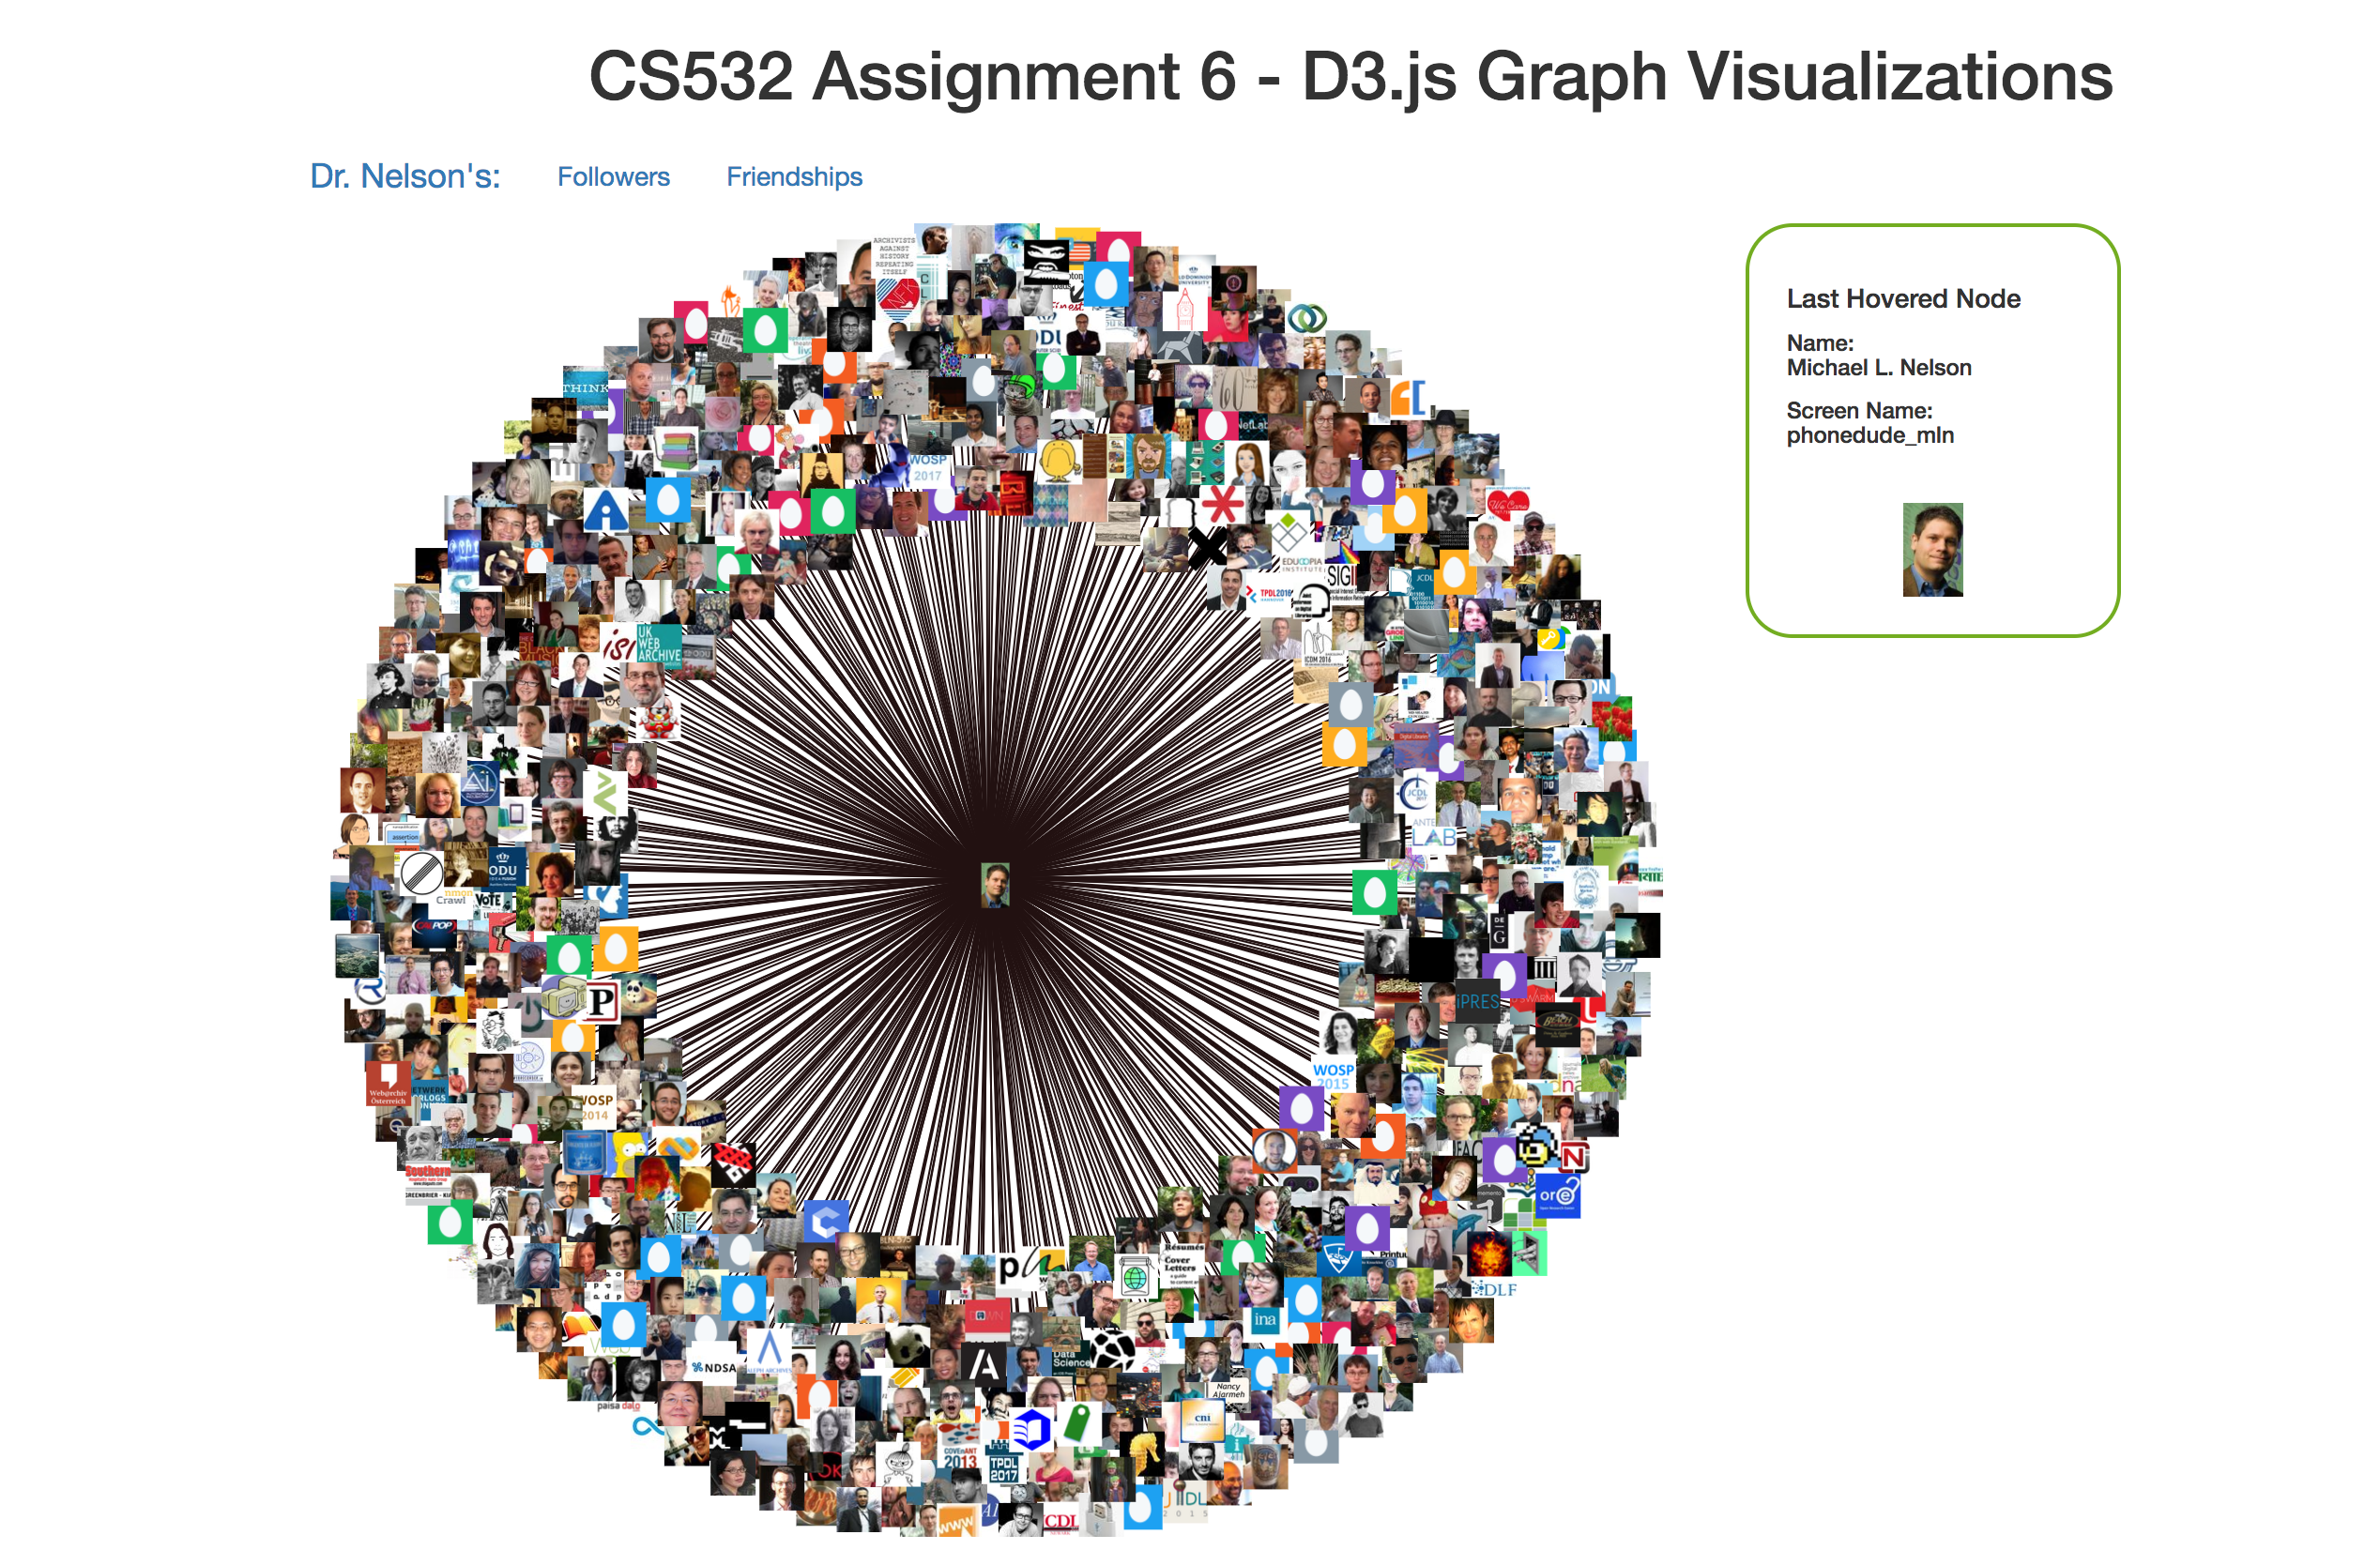
\includegraphics[scale=0.4]{d3followerGraph.png}
 \caption{All of Dr. Nelson's followers in D3 force directed graph}
 \label{fig:q1friendshipgraph}
 \end{figure}


\clearpage

% =================================
% Second question
% =================================

\section*{2}

\subsection*{Question}

\begin{verbatim}
2.  Create an ASCII and JPEG dendrogram that clusters (i.e., HAC)
the most similar blogs (see slides 12 & 13).  Include the JPEG in
your report and upload the ascii file to github (it will be too
unwieldy for inclusion in the report).
\end{verbatim}

\subsection*{Answer}




% \begin{figure}[h]
% \centering
% 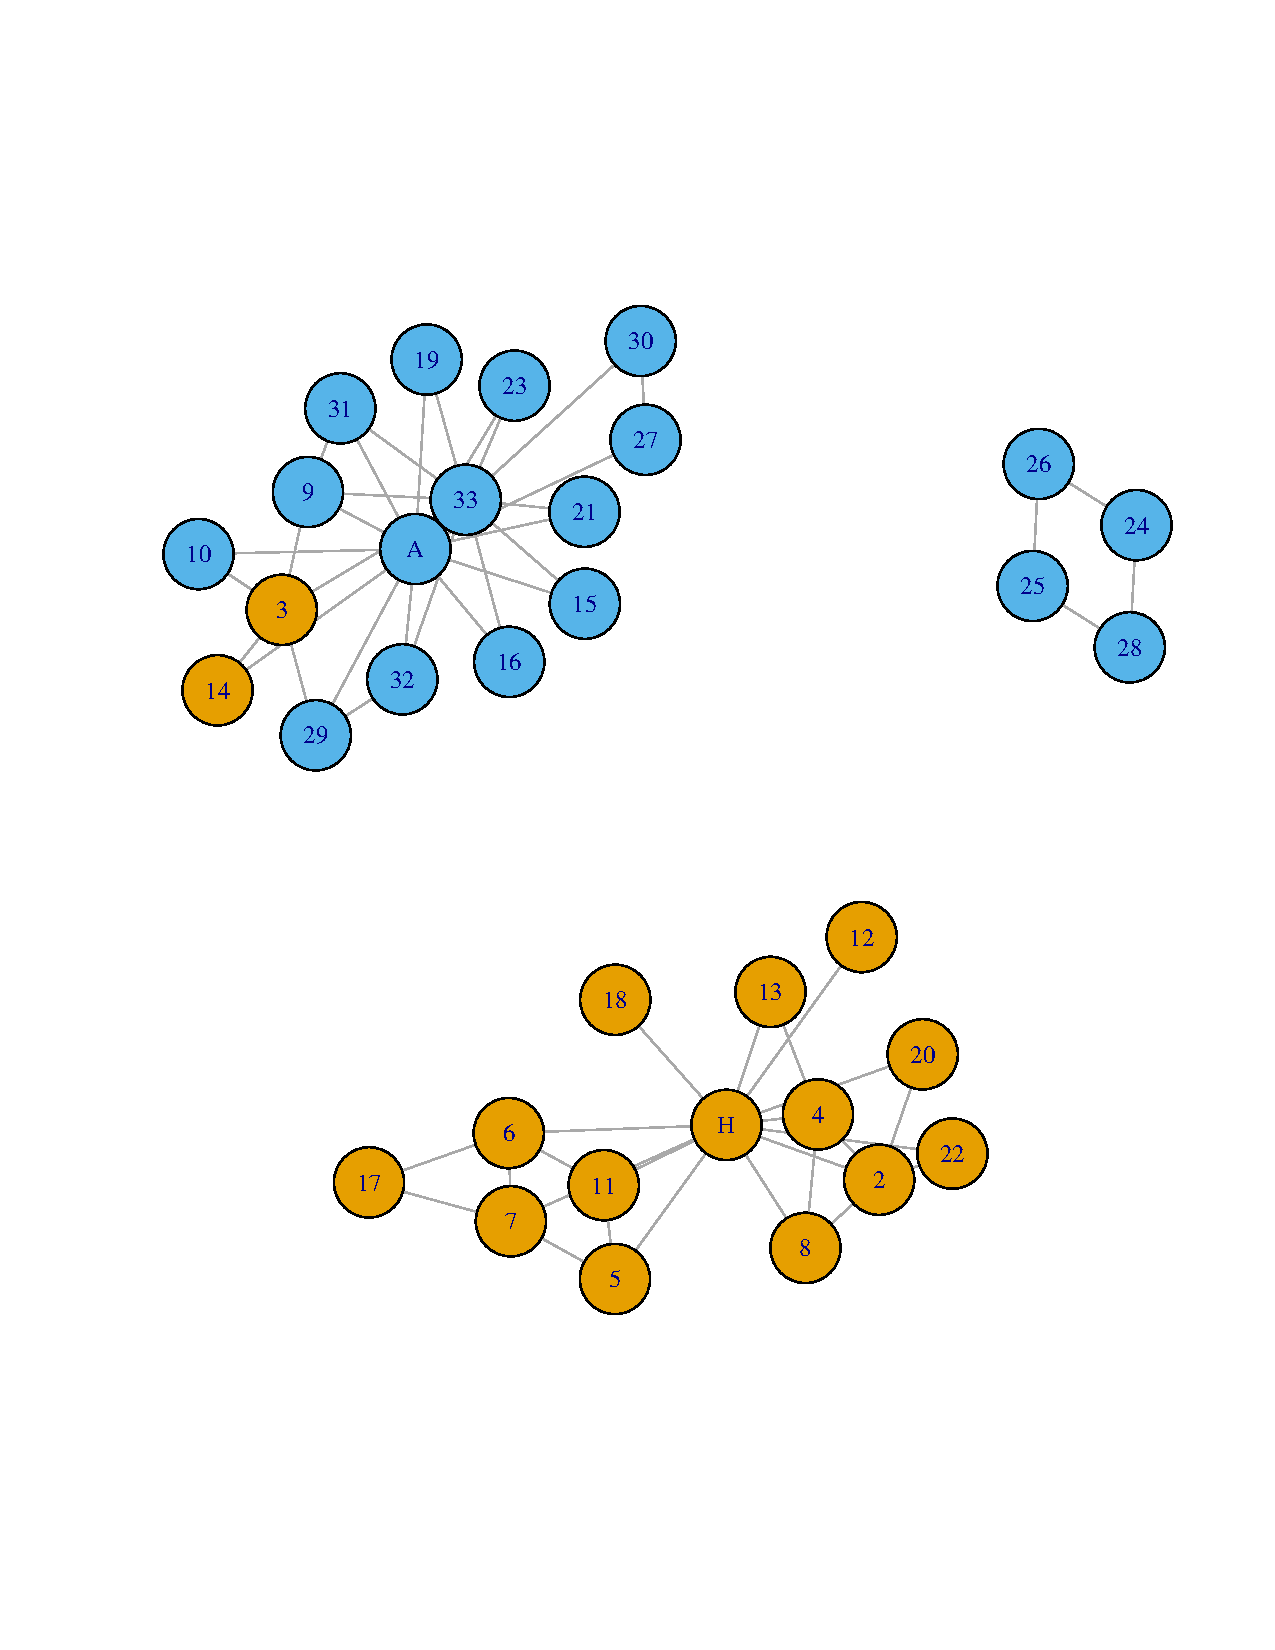
\includegraphics[scale=0.6]{predictedSplit3.pdf}
% \caption{Group split of 3 with Girvan-Newman algorithm from karateClub.R}
% \label{fig:split3}
% \end{figure}

\clearpage

% =================================
% 3rd question
% =================================

\section*{3}

\subsection*{Question}

\begin{verbatim}
3.  Cluster the blogs using K-Means, using k=5,10,20. (see slide
18).  Print the values in each centroid, for each value of k.  How
many interations were required for each value of k?
\end{verbatim}

\subsection*{Answer}

\begin{center}
\Huge{NOT ATTEMPTED}
\end{center}

% \begin{figure}[h]
% \centering
% 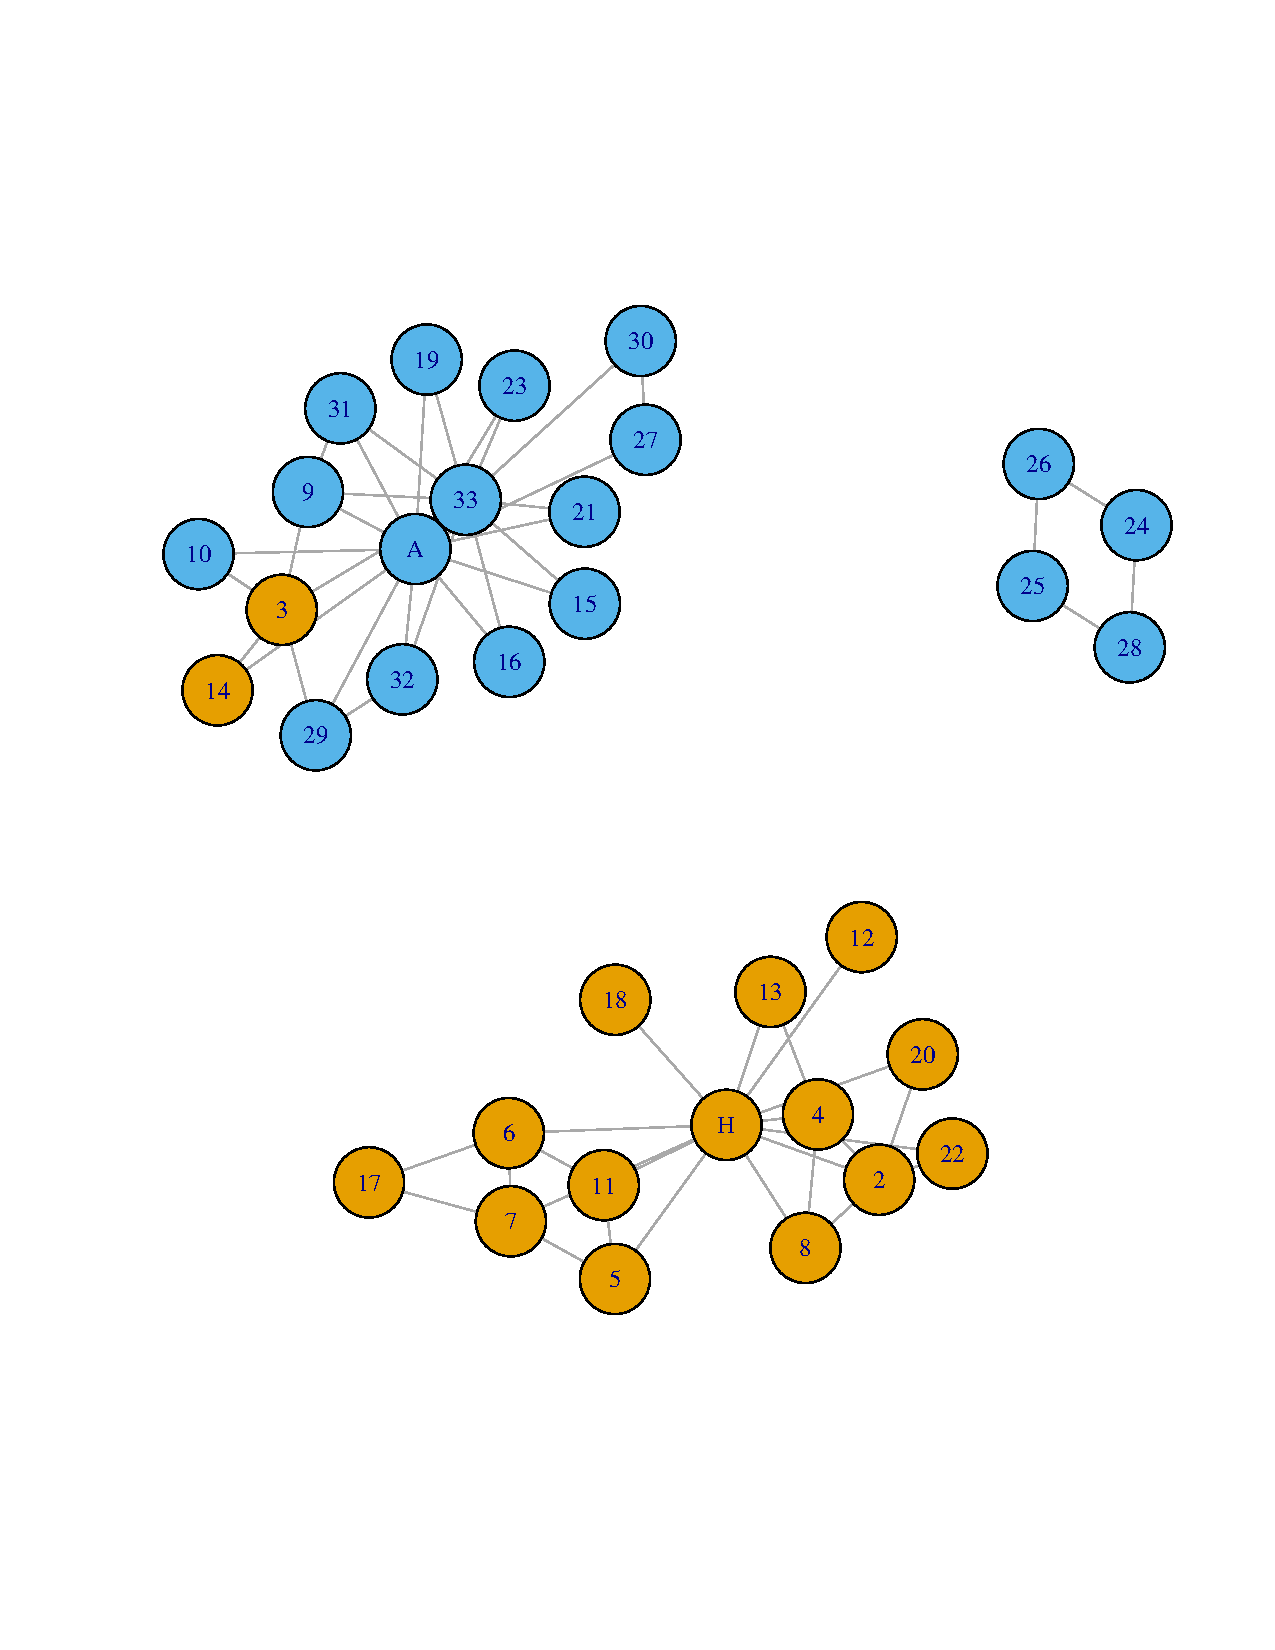
\includegraphics[scale=0.6]{predictedSplit3.pdf}
% \caption{Group split of 3 with Girvan-Newman algorithm from karateClub.R}
% \label{fig:split3}
% \end{figure}


% =================================
% 4th question
% =================================

\section*{4}

\subsection*{Question}

\begin{verbatim}
4.  Use MDS to create a JPEG of the blogs similar to slide 29 of the 
week 12 lecture.  How many iterations were required?
\end{verbatim}

\subsection*{Answer}

\begin{center}
\Huge{NOT ATTEMPTED}
\end{center}

% \begin{figure}[h]
% \centering
% 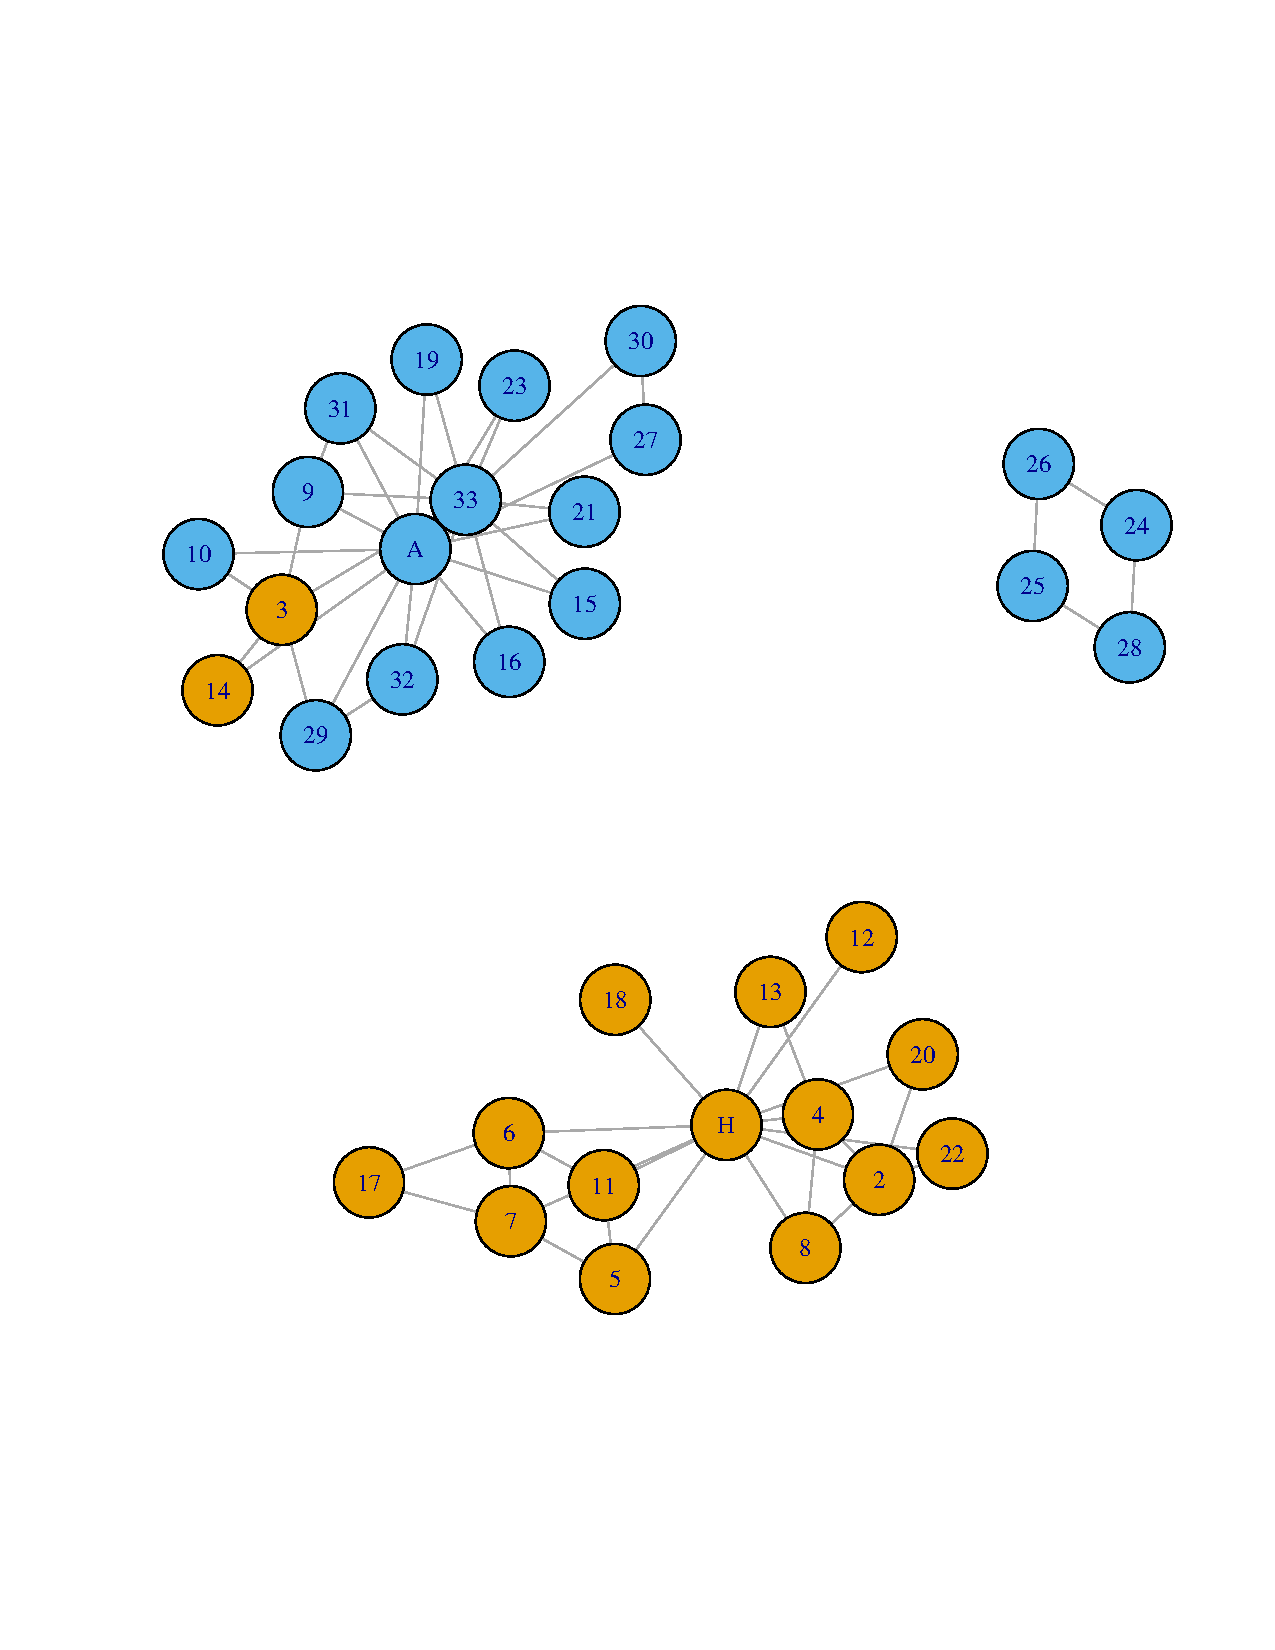
\includegraphics[scale=0.6]{predictedSplit3.pdf}
% \caption{Group split of 3 with Girvan-Newman algorithm from karateClub.R}
% \label{fig:split3}
% \end{figure}

\clearpage

% =================================
% Extra credit
% 5th question
% =================================

\section*{5}

\subsection*{Question}

\begin{verbatim}
5.  Re-run question 2, but this time with proper TFIDF calculations
instead of the hack discussed on slide 7 (p. 32).  Use the same 1000
words, but this time replace their frequency count with TFIDF scores
as computed in assignment #3.  Document the code, techniques,
methods, etc. used to generate these TFIDF values.  Upload the new
data file to github.

Compare and contrast the resulting dendrogram with the dendrogram
from question #2.

Note: ideally you would not reuse the same 1000 terms and instead
come up with TFIDF scores for all the terms and then choose the top
1000 from that list, but I'm trying to limit the amount of work
necessary.
\end{verbatim}

\subsection*{Answer}

\begin{center}
\Huge{NOT ATTEMPTED}
\end{center}

% \begin{figure}[h]
% \centering
% 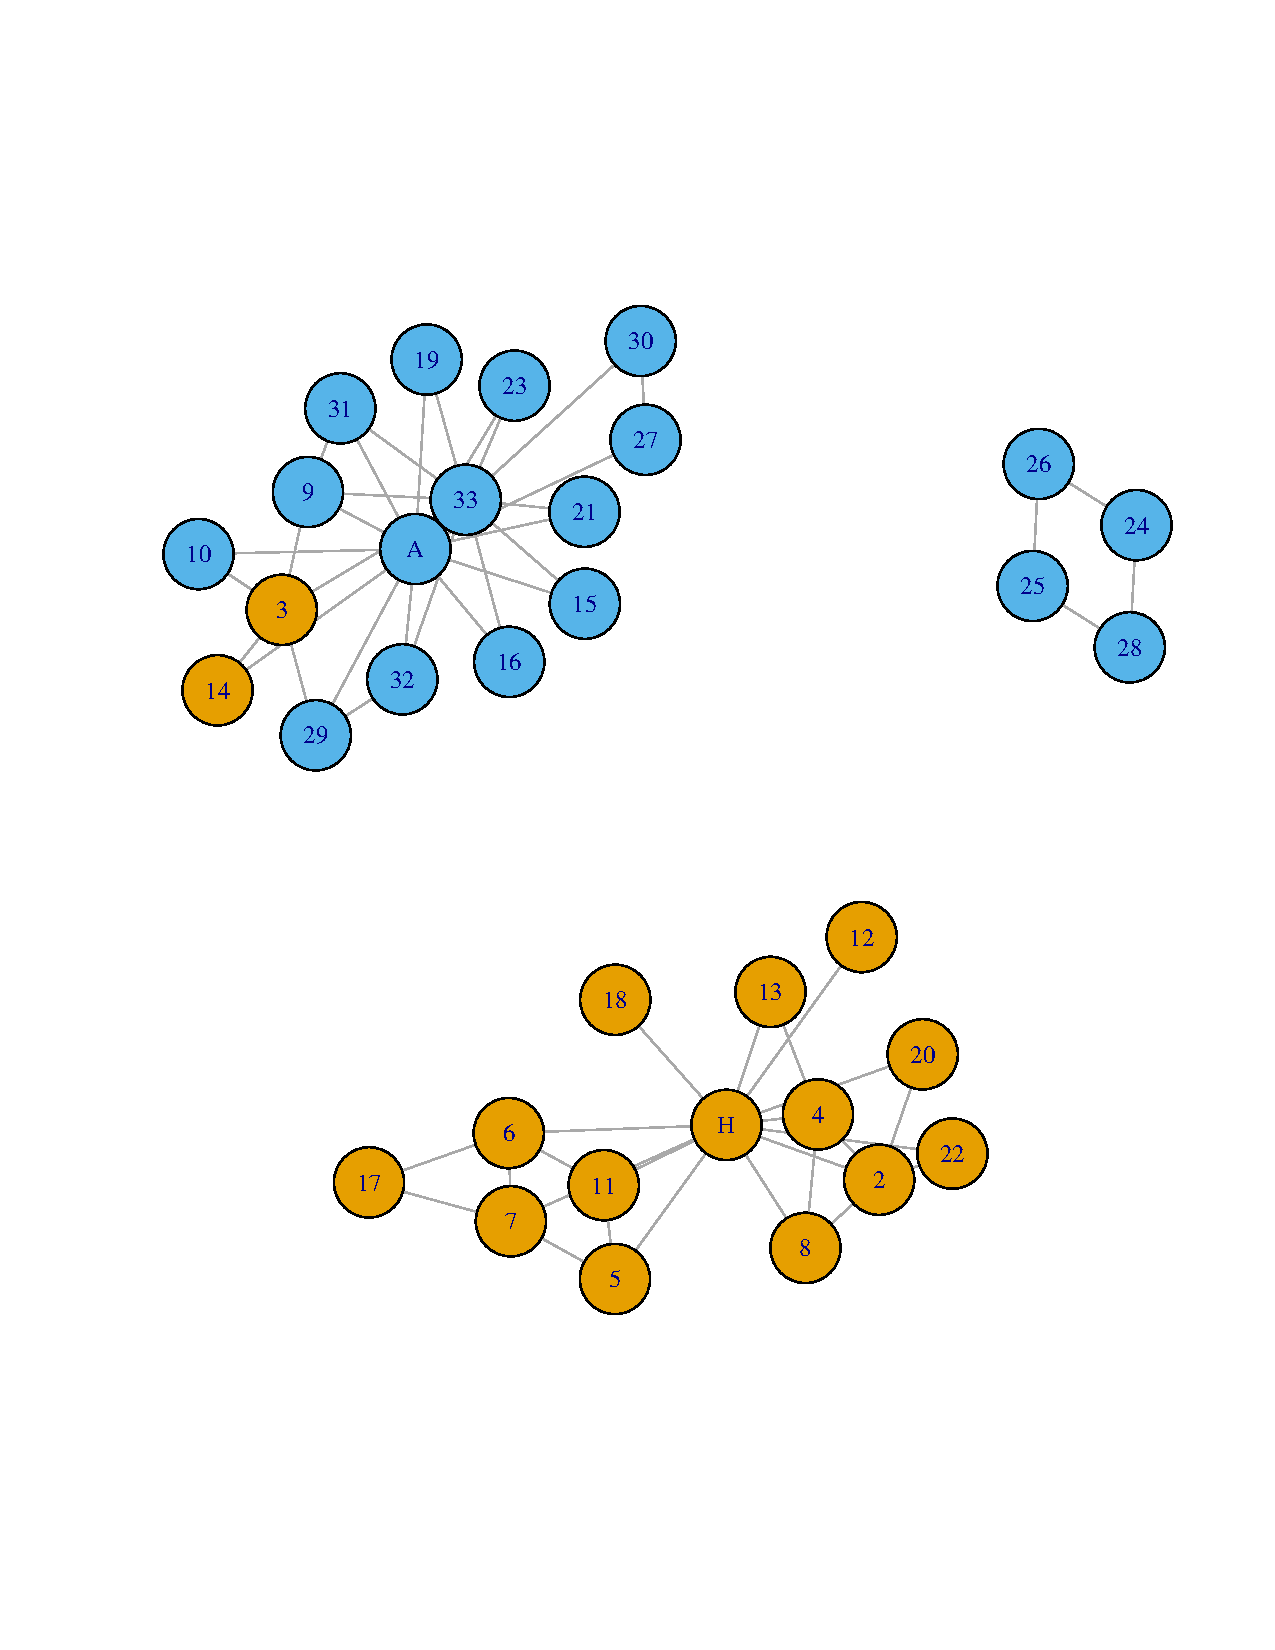
\includegraphics[scale=0.6]{predictedSplit3.pdf}
% \caption{Group split of 3 with Girvan-Newman algorithm from karateClub.R}
% \label{fig:split3}
% \end{figure}

\clearpage

% =================================
% 6th question
% =================================

\section*{6}

\subsection*{Question}

\begin{verbatim}
6.  Re-run questions 1-4, but this time instead of using the 98 
"random" blogs, use 98 blogs that should be "similar" to:

http://f-measure.blogspot.com/
http://ws-dl.blogspot.com/

Choose approximately equal numbers for both blog sets (it doesn't
have to be a perfect 49-49 split, but it should be close).  
Explain in detail your strategy for locating these blogs.  

Compare and contrast the results from the 98 "random" blogs and 
the 98 "targeted" blogs. 
\end{verbatim}

\subsection*{Answer}

\begin{center}
\Huge{NOT ATTEMPTED}
\end{center}


\clearpage


\clearpage


% =================================
% Bibliography
% =================================

\begin{thebibliography}{9}
\bibitem{github}
Atkins, Grant. ``CS532 Assignment 8 Repository'' Github. N.p., 23 March 2017. Web. 23 March 2017.\url{https://github.com/grantat/cs532-s17/tree/master/assignments/A8}.
\bibitem{beautifulsoupref} 
Richardson, Leonard. "Beautiful Soup Documentation." Beautiful Soup Documentation - Beautiful Soup 4.4.0 Documentation. N.p., n.d. Web. 24 Jan. 2017. \url{https://www.crummy.com/software/BeautifulSoup/bs4/doc/}.
\bibitem{collectiveIntell}
Segaran, Toby. ``Programming Collective Intelligence''. O' Reilly, 2007. Web. 6 April 2017. \url{http://shop.oreilly.com/product/9780596529321.do}.
\end{thebibliography}

\end{document}